% TODO: $\Gamma_n^{\Omega}$ is ugly notation. May it's worth to fix it somehow?
% TODO: "parabolic-pseudopotential" to "periodic-pseudopotential".
% TODO: Check all references and labels again.

\chapter{Localized Solutions of Nonlinear Harmonic Oscillator with Periodic Pseudopotential}

\section{Objectives}

In this chapter we study localized solutions of Gross--Pitaevskii equation with a harmonic-oscillator (parabolic) trapping potential and a periodic pseudopotential in front of cubic term.
The effective one-dimensional GPE for mean-fields wave function $\Psi(t, x)$ is
\begin{equation}
	i \Psi_t + \Psi_{xx} - \dfrac{1}{2} a^2 x^2 \Psi + P(x) |\Psi|^2 \Psi = 0,
\label{eq:gpe-parabolic-non-scaled}
\end{equation}
where $a^2$ is the strength of the harmonic-oscillator potential, and pseudopotential $P(x)$ is a function of period $L = 2 \pi / \Omega$:
\begin{equation}
	P(x + 2 \pi / \Omega) = P(x).
\end{equation}
Such model can be achieved by means of combination of a magnetic trap and an optical lattice which induces the periodic pseudopotential via the Feshbach resonance \cite{SakaguchiMalomed2010}.
Intervals with positive (negative) values of $P(x)$ correspond to spatial domains with attractive (repulsive) interactions between particles.

The model includes {\it two scales}: the characteristic harmonic-oscillator length $l_{\mathrm{HO}} \sim 1 / \sqrt{a}$, and period $L = 2 \pi / \Omega$ of the pseudopotential.
In particular, the limit case of the wide harmonic-oscillator trap $\Omega \gg 2 \pi \sqrt{a}$, is a physically relevant one.
Let's introduce additional rescaling
\begin{equation}
	t \to \dfrac{a}{\sqrt{2}} t, \quad x \to \dfrac{\sqrt{a}}{\sqrt[4]{2}} x, \quad \Psi \to \dfrac{\sqrt[4]{2}}{\sqrt{a}} \Psi.
\end{equation}
This allows to fix $a \equiv 1$ and convert \eqref{eq:gpe-parabolic-non-scaled} into a normalized form
\begin{equation}
	i \Psi_t + \Psi_{xx} - x^2 \Psi + P(x) |\Psi|^2 \Psi = 0,
\label{eq:gpe-parabolic}
\end{equation}
where $P(x)$ is periodic with spatial frequency $\widetilde{\Omega} = \Omega / \sqrt{a}$.
In what follows below, symbol $\widetilde{\Omega}$ is replaced by $\Omega$.
To estimate physically relevant values of $\Omega$ we use the results of experimental realization of the periodically-modulated Feshbach resonance in \cite{YamazakiTaieSugawaTakahashi}.
There the corresponding scaled spatial frequency being $\Omega \sim 100$.
It can be made smaller, taking larger $a$.

Equation \eqref{eq:gpe-parabolic} is our basic model.
The objective of our analysis is to study its localized stationary solutions of the form
\begin{equation}
	\Psi(t, x) = u(x) e^{-i \omega t},
\end{equation}
where real-valued function $u(x)$ satisfies equation
\begin{equation}
	u_{xx} + (\omega - x^2) u + P(x) u^3 = 0
\label{eq:nho-periodic}
\end{equation}
with localization boundary conditions
\begin{equation}
	\lim \limits_{x \to \pm \infty} u(x) = 0.
\end{equation}
During our numerical analysis we focus on the practically important case when the pseudopotential function $P(x)$ in \eqref{eq:gpe-parabolic} is taken as a sum of constant and harmonic parts of a prototypical cosine form:
\begin{equation}
	P(x) = P_0 + P_1 \cos (\Omega x).
\label{eq:gpe-parabolic-pseudopotential}
\end{equation}

As we say it in Chapter~\ref{chapter:III} stability of solutions is a critically important property.
Linear stability of localized solutions is addressed by considering of small perturbations of a solution $u(x)$ of the form:
\begin{equation}
	\Psi(t, x) = \left( u(x) + (v(x) + w(x)) e^{\lambda t} + (v^{\dagger}(x) - w^{\dagger}(x)) e^{\lambda^{\dagger} t} \right) e^{-i \omega t},
\label{eq:gpe-parabolic-perturabation}
\end{equation}
where $|v(x)| \ll 1$, $|w(x)| \ll 1$.
Substituting \eqref{eq:gpe-parabolic-perturabation} into \eqref{eq:gpe-parabolic} and performing linearization with respect to $v(x)$ and $w(x)$, we arrive at eigenvalue problem
\begin{equation}
	i
	\begin{pmatrix}
		0 & \mathcal{L}_- \\
		\mathcal{L}_+ & 0
	\end{pmatrix}
	\begin{pmatrix}
		v \\ w
	\end{pmatrix} =
	\lambda
	\begin{pmatrix}
		v \\ w	
	\end{pmatrix},
\label{eq:eigenvalue-problem-gpe-parabolic}
\end{equation}
where 
\begin{eqnarray*}
	&& \mathcal{L}_- = \partial_{xx} + \omega -x^2 + P(x) u^2; \\
	&& \mathcal{L}_+ = \partial_{xx} + \omega -x^2 + 3 P(x) u^2.
\end{eqnarray*}
This problem is similar to the previously considered problem \eqref{eq:eigenvalue-problem}.
Fourier Collocation Method from Chapter~\ref{chapter:III} is also applicable for effective numerical evaluation of spectrum \eqref{eq:eigenvalue-problem-gpe-parabolic}.
Eigenvalues with non-zero real part rise to the instability, while pure imaginary spectrum indicates that solutions is linearly stable.
Again, we note that the eigenvalues appears in pairs and quadruples, i.e. if $\lambda$ is an eigenvalue, then $-\lambda$, $\lambda^{\dagger}$, $-\lambda^{\dagger}$ are eigenvalues too.

For the analytical analysis during this chapter it's convenient to rewrite eigenvalue problem \eqref{eq:eigenvalue-problem-gpe-parabolic} in the equivalent form:
\begin{equation}
	\mathcal{L}_+ \mathcal{L}_- w = \Lambda w, \quad \Lambda = -\lambda^2.
\label{eq:eigenvalue-problem-gpe-parabolic-analytical}
\end{equation}
In terms of \eqref{eq:eigenvalue-problem-gpe-parabolic-analytical}, a solution $u(x)$ passes the linear stability test if the spectrum of eigenvalues $\Lambda$ is all-real positive.

\subsection{Solutions with linear counterpart}

An important class of localized solutions of equation \eqref{eq:nho-periodic} is {\it nonlinear solutions with linear counterpart}.
Such terminology has been adopted in \cite{AgostaMalomedPresilla, AgostaPresilla}.
Existence of such solution came from the consideration of the low-amplitude limit.
% TODO: Add reference to the definition of norm from the overall introduction, not from Chapter III.
For a small value of norm $N$, see \eqref{eq:norm}, the nonlinear term in \eqref{eq:nho-periodic} may be neglected, which leads to the ordinary harmonic-oscillator equation
\begin{equation}
	u_{xx} + (\omega - x^2) u = 0.
\label{eq:ho}
\end{equation}
Equation \eqref{eq:ho} produces the commonly known set of eigenvalues and eigenfunctions:
\begin{equation}
	\tilde{\omega}_n = 2n + 1; \quad \tilde{u}_n(x) = \dfrac{1}{\sqrt{2^n n! \sqrt{\pi}}} H_n(x) e^{-\frac{-1}{2} x^2}; \quad n = 0, 1, \dots,
\label{eq:ho-solutions}
\end{equation}
where $H_n(x)$ functions are Hermite polynomials.
In particular,
\begin{equation*}
	H_0(x) = 1, \quad H_1(x) = 2x, \quad H_2(x) = 4x^2 - 2.	
\end{equation*}

When the nonlinearity is switched on, each linear eigenstate $(\tilde{\omega}_n, \tilde{u}_n(x))$ bifurcates into a one-parameter set $\Gamma_n = (\omega_n, u_n(x))$ of small-amplitude localized solutions of \eqref{eq:nho-periodic}.
These solutions are produced by equation \eqref{eq:nho-periodic} and become essentially nonlinear with the increase of $N$ and distance between $\omega_n$ and $\tilde{\omega}_n$.
Localized solutions from family $\Gamma_n$ feature the same parity as the corresponding linear eigenfunction $\tilde{u}_n(x)$, solution with even $n$ are even functions of $x$, and those with the odd $n$ are odd.
Localized solution with $n = 0$ originates form the ground state of the harmonic-oscillator.

During our analysis it's interesting to compare the results with the well-studied case of Gross--Pitaevskii equation \eqref{eq:gpe-parabolic} with constant $P(x)$ (negative or positive).
In this case $P_1 \equiv 0$ in \eqref{eq:gpe-parabolic-pseudopotential}, and after additional rescaling $\Psi \to \Psi / \sqrt{|P_0|}$ equation \eqref{eq:nho-periodic} takes form
\begin{equation}
	u_{xx} + (\omega - x^2) u + \sigma_0 u^3 = 0,
\label{eq:nho}
\end{equation}
where $\sigma_0 = P_0 / |P_0| = \mathrm{sign}(P_0)$.
Let's call equation \eqref{eq:nho} the {\it nonlinear harmonic-oscillator equation with constant pseudopotential} (we also refer to this equation simply as {\it nonlinear harmonic-oscillator}).
The case $\sigma_0 = 1$ ($\sigma_0 = -1$) corresponds to the attractive (repulsive) interparticle interactions.
It's convenient to illustrate branches of localized solutions of equation \eqref{eq:nho} by means of respective $N(\omega)$ curves, which are presented in Figure~\ref{fig:branches-nho}, as per \cite{ZezyulinAlfimovKonotopPerecGarcia2007, ZezyulinAlfimovKonotopPerecGarcia2008} for the cases $\sigma_0 = \pm 1$.
The branches $\Gamma_n$, $n = 0, 1, \dots$, correspond to the solutions with linear counterparts, bifurcating from them at the points $\tilde{\omega}_n = 2n + 1$, $N = 0$.
All the branches being represented by monotonous functions $N(\omega)$.
Other results obtained for localized solutions of \eqref{eq:nho} can be presented as follows.
\begin{itemize}
	\item Presumably, there exist no nonlinear solutions of \eqref{eq:nho} without linear counterpart \cite{AlfimovZezyulin}.
	\item Solutions corresponding to families $\Gamma_0$, $\Gamma_1$ are stable in the small-amplitude limit and for moderate and large amplitudes as well for both cases $\sigma_0 = \pm 1$.
	\item
		The small-amplitude solutions belonging to the branch $\Gamma_2$ are unstable.
		For the case $\sigma_0 = 1$, the instability of the branch $\Gamma_2$ persists for $\omega^* < \omega < 5$, where $\omega^* \approx 3.83$.
		According to the numerical study at $\omega < \omega^*$ these solutions was reported to be stable \cite{AlfimovZezyulin}.
		For the case $\sigma_0 = -1$ the branch $\Gamma_2$ is fully unstable. 
\end{itemize}

\begin{figure}[h]
\centering
	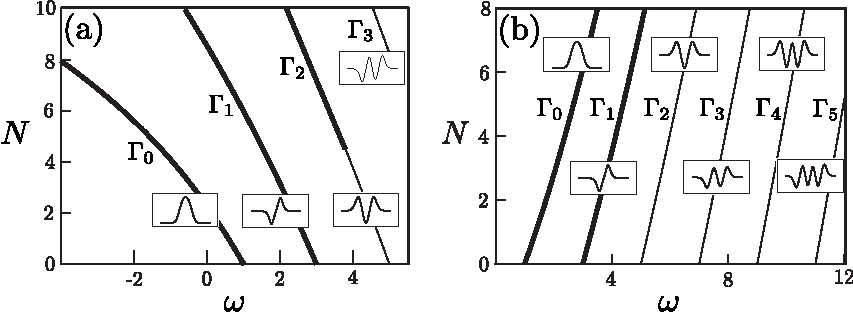
\includegraphics[scale = 1]{pic/stability for nho with constant pseudopotential}
	\caption{
		$N(\omega)$ curves for equation \eqref{eq:nho}, with (a) $\sigma_0 = 1$, (b) $\sigma_0 = -1$.
		Bold (thin) segments correspond to stable (unstable) solutions.
		Insets show schematic profiles of solutions $u_n(x)$ from each family $\Gamma_n$.
	}
\label{fig:branches-nho}
\end{figure}

Before we can move on let's briefly resume our goals in this chapter.
We study localized solutions of equation \eqref{eq:gpe-parabolic} with periodic pseudopotential \eqref{eq:gpe-parabolic-pseudopotential}.
We apply linear stability analysis to find stable solutions among them.
Our baseline model for comparison is well-studied equation \eqref{eq:nho} for nonlinear harmonic-oscillator with constant pseudopotential.
We pay special attention to the localized solutions with linear counterpart, and study how the presence of periodic pseudopotential $P(x)$ of the cosine form \eqref{eq:gpe-parabolic-pseudopotential} affects their stability.

\section{Small-Amplitude Localized Solutions with Linear Counterpart}

For Eq.~\eqref{eq:nho-periodic} let's consider a small-amplitude limit of solutions with linear counterpart.
As we say above, such solutions $u_n(x)$ originate from the bifurcation of eigenstates $(\tilde{\omega}_n, \tilde{u}_n(x))$ of harmonic-oscillator equation \eqref{eq:ho} and form families $\Gamma_n = (\omega_n, u_n(x))$.
If the amplitude of $u_n(x)$ is small the localized solutions from branch $\Gamma_n$ are approximated by expansions \cite{ZezyulinAlfimovKonotopPerecGarcia2008},
\begin{equation}
	u_n(x) = \varepsilon \tilde{u}_n(x) + o(\varepsilon), \quad \omega_n = \tilde{\omega}_n - \varepsilon^2 \Delta_n + o(\varepsilon^2),
\label{eq:small-amplitude-expansion}
\end{equation}
where $\varepsilon \ll 1$ is a small parameter, and
\begin{equation}
	\Delta_n = \int \limits_{-\infty}^{+\infty} P(x) \tilde{u}_n^4(x) dx = \dfrac{1}{2^{2n} (n!)^2 \pi} \int \limits_{-\infty}^{+\infty} P(x) H_n^4(x) e^{-2x^2} dx.
\label{eq:Delta_n}
\end{equation}

Let's address stability of these small-amplitude solutions.
We note that with the help of expansion \eqref{eq:small-amplitude-expansion}, operator $\mathcal{L}_+ \mathcal{L}_-$ in \eqref{eq:eigenvalue-problem-gpe-parabolic-analytical} may be considered as a perturbation of operator $\mathcal{L}_n^2$, where
\begin{equation}
	\mathcal{L}_n = \partial_{xx} + 2n + 1 - x^2.
\end{equation}
Specifically,
\begin{eqnarray*}
	&& \mathcal{L}_+ = \mathcal{L}_n + \varepsilon^2 (3 P(x) \tilde{u}_n^2(x) - \Delta_n) + o(\varepsilon^2); \\
	&& \mathcal{L}_- = \mathcal{L}_n + \varepsilon^2 (P(x) \tilde{u}_n^2(x) - \Delta_n) + o(\varepsilon^2).
\end{eqnarray*}
% TODO: Consider to use $\mathcal{M}_n$ instead of $M_n$.
So, for the operator $\mathcal{L}_+ \mathcal{L}_-$ we can write
\begin{equation}
	\mathcal{L}_+ \mathcal{L}_- = \mathcal{L}_n^2 + \varepsilon^2 M_n + o(\varepsilon^2),
\label{eq:perturbed-operator}
\end{equation}
where
\begin{equation}
	M_n = (2 P(x) \tilde{u}_n^2(x) - \Delta_n) \mathcal{L}_n + \mathcal{L}_n (P(x) \tilde{u}_n^2(x) - \Delta_n).
\label{eq:Mn}
\end{equation}
Operator $\mathcal{L}_n$ is self-adjoint in $L^2$ space, and its spectrum consists of eigenvalues $\varkappa_k = 2(n - k)$ with corresponding eigenfunctions $\tilde{u}_k(x)$, $k = 0, 1, \dots$  in the form \eqref{eq:ho-solutions}.
The spectrum is equidistant, all the eigenvalues being simple.
There are infinitely many negative eigenvalues, $n$ positive eigenvalues, and one zero eigenvalue.
The eigenvalues $\widetilde{\Lambda}_k$ of operator $\mathcal{L}_n^2$ are squared eigenvalues of $\mathcal{L}_n$, i.e. $\widetilde{\Lambda}_k = \varkappa_k^2 = 4 (k - n)^2$, corresponding to the same eigenfunctions $\tilde{u}_k(x)$.
This means that the spectrum of $\mathcal{L}_n^2$ includes $n$ {\it double positive eigenvalues} $\widetilde{\Lambda}_k = 4 (n - k)^2$, $k = 0, 1, \dots, (n - 1)$, one {\it simple zero eigenvalue} and {\it infinitely many simple positive eigenvalues}.
Each of the double eigenvalues has an invariant subspace spanned by two functions, $\tilde{u}_k(x)$ and $\tilde{u}_{2n - k}(x)$.
If $n = 0$, then all eigenvalues of $\mathcal{L}_n^2$ are simple.

Generically, small perturbation of $\mathcal{L}_n$ results in {\it splitting} of the double eigenvalues.
Each of them can split into (i) two real eigenvalues of the perturbed operator or (ii) two complex-conjugate eigenvalues.
If the case (i) takes place for each double eigenvalue, then small-amplitude localized solutions bifurcating form the $n$-th linear eigenstate are marginally stable, at least in some vicinity of the bifurcation.
However, if at least for one double eigenvalue the case (ii) takes place, then the bifurcating small-amplitude solutions  are unstable in vicinity of the bifurcation.

To address the splitting of double eigenvalues when passing from operator $\mathcal{L}_n^2$ to the perturbed one, $\mathcal{L}_+ \mathcal{L}_-$ in \eqref{eq:perturbed-operator}, we construct an {\it asymptotic expansion for perturbed eigenvalues} following \cite{ZezyulinAlfimovKonotopPerecGarcia2008}.
Under the actions of the perturbation, each double eigenvalue $\widetilde{\Lambda}_k$ splits into two simple ones:
\begin{equation}
	\Lambda_{k, 1} = \widetilde{\Lambda}_k + \varepsilon^2 \gamma_1 + o(\varepsilon^2), \quad \Lambda_{k, 2} = \widetilde{\Lambda}_k + \varepsilon^2 \gamma_2 + o(\varepsilon^2),
\label{eq:eigenvalues-split}
\end{equation}
where the coefficients $\gamma_{1,2}$ are the eigenvalues of the 2$\times$2 matrix
\begin{equation}
	\widetilde{M}_n =
	\begin{pmatrix}
		\langle M_n \tilde{u}_k, \tilde{u}_k \rangle & \langle M_n \tilde{u}_k, \tilde{u}_{2n - k} \rangle \\
		\langle M_n \tilde{u}_{2n - k}, \tilde{u}_k \rangle & \langle M_n \tilde{u}_{2n - k}, \tilde{u}_{2n - k} \rangle
	\end{pmatrix}.
\label{eq:M}
\end{equation}
Therefore, if the eigenvalues of $\widetilde{M}_n$ are real for each $k = 0, 1, \dots, n - 1$, then the spectrum of $\mathcal{L}_+ \mathcal{L}_-$ remains real and the nonlinear localized solution $u_n(x)$ is stable, at least for sufficiently small $\varepsilon$.
Otherwise, if eigenvalues of $\widetilde{M}_n$ are complex for some $k = 0, 1, \dots, n - 1$, then solution $u_n(x)$ is unstable in a vicinity of the bifurcation.
None that, as no double eigenvalues exist for $n = 0$, the small-amplitude solutions of the family $\Gamma_0$ are stable for any $P(x)$.

Using explicit expressions for the eigenfunctions $\tilde{u}_n(x)$ from \eqref{eq:small-amplitude-expansion} and expressions for $M_n$ from \eqref{eq:Mn}, one can compute the entries of the matrix $\widetilde{M}_n$:
\begin{align}
\langle M_n \tilde{u}_k &, \tilde{u}_k \rangle = \frac{8(n-k)}{\pi 2^{(n+k)} n! k!} \int \limits_{-\infty }^{+\infty} P(x) H_n^2(x) H_k^2(x) e^{-2 x^2} dx \notag \\ & - \frac{4(n-k)}{\pi 2^{2n}(n!)^2} \int \limits_{-\infty }^{+\infty} P(x) H_n^4(x) e^{-2 x^2} dx; \label{eq:Mn11} \\
\langle M_n \tilde{u}_k &, \tilde{u}_{2n-k} \rangle = -\langle M_n \tilde{u}_{2n-k}, \tilde{u}_k \rangle = \notag \\ & = \frac{4 (n-k)}{\pi 2^{2n} n! \sqrt{k! (2n-k)!}} \int \limits_{-\infty}^{+\infty} P(x) H_n^2(x) H_{2n-k}(x) H_k(x) e^{-2 x^2} dx;  \label{eq:Mn12} \\
\langle M_n \tilde{u}_{2n-k} &, \tilde{u}_{2n-k} \rangle = -\frac{8(n-k)}{\pi 2^{(3n-k)} n! (2n-k)!} \int \limits_{-\infty}^{+\infty} P(x) H_n^2(x) H_{2n-k}^2(x) e^{-2 x^2} dx \notag \\ & + \frac{4(n-k)}{\pi 2^{2n} (n!)^2} \int \limits_{-\infty}^{\infty} P(x) H_n^4(x) e^{-2 x^2} dx. \label{eq:Mn22}
\end{align}
Formulas \eqref{eq:Mn11} -- \eqref{eq:Mn22} with $P(x) = \pm 1$ were used in \cite{ZezyulinAlfimovKonotopPerecGarcia2008} to explore the stability of small-amplitude nonlinear solutions in the model with constant pseudopotential.

\section{Branches of Nonlinear Localized Solutions for Periodic Pseudopotential, $P(x) = P_0 + P_1 \cos (\Omega x)$}

We present our numerical and analytical results for pseudopotential of the cosine form \eqref{eq:gpe-parabolic-pseudopotential}.
It represents a sum of a constant part $P_0$ and a periodic part $P_1 \cos (\Omega x)$.
In what follow below we conclude that the relation between the magnitudes of $|P_0|$ and $|P_1|$ is important.
Hence, it's necessary to consider two cases separately: (a) $|P_0| \gtrsim |P_1|$, when the constant component is not negligible, and (b) $|P_0| \ll |P_1|$, when the constant component is negligible and pseudopotential \eqref{eq:gpe-parabolic-pseudopotential} should be treated as a function with zero mean. 
We consider each of these cases separately.

\subsection{Periodic pseudopotential with Non-Zero Mean, $|P_0| \gtrsim |P_1|$}

If $P_0$ component of pseudopotential is not negligible, one can scale out the absolute value of it, by replacing 
\begin{equation}
	\Psi \to \Psi / \sqrt{|P_0|}, \quad P_1 / |P_0| \to P_1.
\end{equation}
Equation \eqref{eq:gpe-parabolic} takes form
\begin{equation}
	i \Psi_t + \Psi_{xx} + x^2 \Psi + (\sigma_0 + P_1 \cos (\Omega x)) |\Psi|^2 \Psi = 0.
\label{eq:gpe-non-zero-mean}
\end{equation}
where $\sigma_0 \equiv P_0 / |P_0| = \mathrm{sign} (P_0)$.
Stationary states equation in this case has form
\begin{equation}
	u_{xx} + (\omega - x^2) u + (\sigma_0 + P_1 \cos (\Omega x)) u^3 = 0.
\label{eq:nho-non-zero-mean}
\end{equation}
A generic picture of localized solutions of equation \eqref{eq:nho-non-zero-mean} can be obtained by means of a numerical shooting algorithm.
A representative example of the respective $N(\omega)$ curves with $\sigma_0 = 1$, $P_1 = 2$ (which implies that the sign of the pseudopotential periodically flips), and $\Omega = 12$ is displayed in Figure~\ref{fig:branches-nho-periodic-attractive}.
One can immediately observe that, apart from branches $\Gamma_n$ originating from their linear counterparts, numerous branches of localized solutions {\it without linear counterpart} exist too.
Thus, the presence of the periodic component in the pseudopotential essentially enriches the diversity of available solutions.
This contrasts with the case of nonlinear harmonic-oscillator with constant pseudopotential, see Figure~\ref{fig:branches-nho}.
However, we did not find stable solutions without linear counterpart.
On Figure~\ref{fig:branches-nho-periodic-attractive} the only stables solutions correspond to branches $\Gamma_0$, $\Gamma_1$, $\Gamma_2$.

\begin{figure}[h]
\centering
	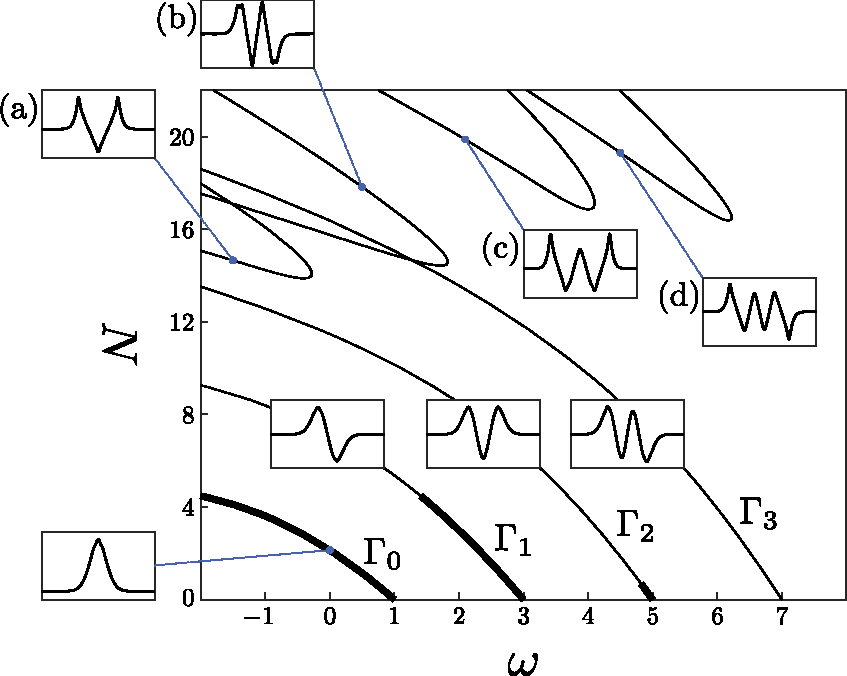
\includegraphics[scale = 1]{pic/branches for cosine nho, case (a)}
	\caption{
		Curves $N(\omega)$ of localized solution families for equation \eqref{eq:nho-non-zero-mean} with non-zero mean cosine pseudopotential with $\sigma_0 = 1$, $P_1 = 2$, and $\Omega = 12$.
		Thin and bold lines show unstable and stable solution families.
		Branches $\Gamma_n$, $n = 0, 1, 2, 3$ represent solutions with linear counterpart.
		Insets on top and outside of the branches are representative profiles $u(x)$ of solutions obtained from the corresponding families.
		Branches (a), (b), (c), and (d) represent solutions without linear counterpart.
		All of them were found to be unstable.
	}
\label{fig:branches-nho-periodic-attractive}
\end{figure}

Similar situation takes place for $\sigma_0 = -1$, while all other parameters remain the same, $P_1 = 2$ and $\Omega = 12$.
Respective $N(\omega)$ curves are presented in Figure~\ref{fig:branches-nho-periodic-repulsive}.
Localized solutions without linear counterpart correspond to branches (a) and (b).
Branches $\Gamma_0$, $\Gamma_1$ have stability regions.
All other families were found to be unstable.

\begin{figure}[h]
\centering
	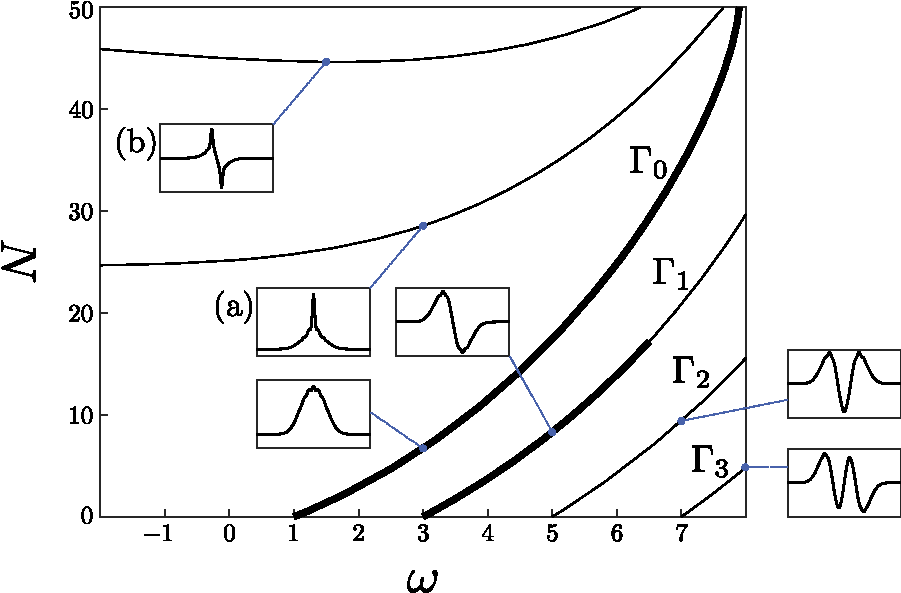
\includegraphics[scale = 1]{pic/branches for cosine nho, case (b)}
	\caption{
		Curves $N(\omega)$ of localized solution families for equation \eqref{eq:nho-non-zero-mean} with non-zero mean cosine pseudopotential with $\sigma_0 = -1$, $P_1 = 2$, and $\Omega = 12$.
		Thin and bold lines show unstable and stable solution families.
		Branches $\Gamma_n$, $n = 0, 1, 2, 3$ represent solutions with linear counterpart, two of them, $\Gamma_0$ and $\Gamma_1$, have regions of stability.
		All other families are unstable.
		Insets with blue dashed lines represent profiles $u(x)$ of the solutions.
	}
\label{fig:branches-nho-periodic-repulsive}
\end{figure}

In the limit of the rapidly oscillation of $P(x)$, $\Omega \to \infty$, localized solutions of \eqref{eq:nho-non-zero-mean} may be approximated by solutions of nonlinear harmonic-oscillator equation with constant pseudopotential \eqref{eq:nho}.
The asymptotic formula can be obtained by means of averaging with respect to fast oscillations (see, e.g. \cite{AbdullaevCaputoKraenkelMalomed}):
\begin{equation}
	u(x) = v(x) + \frac{1}{\Omega^2} \bigg( w(x) + P_1 w^3(x) \cos (\Omega x) \bigg) + o \bigg( \frac{1}{\Omega^2} \bigg), \quad \Omega \to \infty.
\label{eq:nho-non-zero-mean-asymptotic}
\end{equation}
Here $v(x)$ is a solution of Eq.~\eqref{eq:nho}, and $w(x)$ is a localized solution of the linear equation
\begin{equation}
	w_{xx} + (\omega - x^2 + 3 \sigma_0 v^2(x)) w = -\frac{3}{2} P_1^2 v^5(x).
\end{equation}
We stress that asymptotic relation \eqref{eq:nho-non-zero-mean-asymptotic} is valid for nonlinear solutions of arbitrary amplitudes (i.e. not only in the small-amplitude limit), provided that $\Omega^2$ is large enough.

\begin{figure}[h]
\centering
	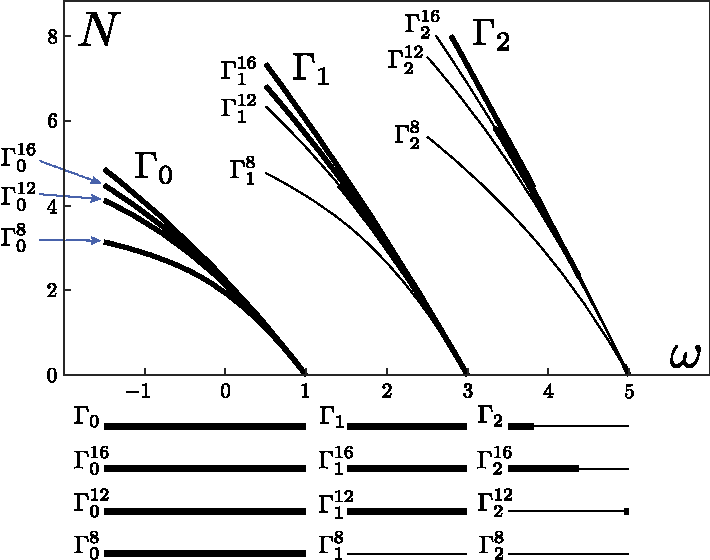
\includegraphics[scale = 1]{pic/branches with linear counterpart, non-zero mean cosine nho}
	\caption{
		Curves $N(\omega)$ of branches $\Gamma_n^{\Omega}$ for equation \eqref{eq:nho-non-zero-mean} with $\sigma_0 = 1$, $P_1 = 2$, and $\Omega = 8, 12, 16$.
		Only branches with $n = 0, 1, 2$ are shown.
		For comparison, the corresponding dependencies $\Gamma_n$ for nonlinear harmonic-oscillator \eqref{eq:nho} for the case $\sigma_0 = 1$ are show too.
		These curves are identical to those in Figure~\ref{fig:branches-nho}~(a).
		According to \eqref{eq:nho-non-zero-mean-asymptotic} branches $\Gamma_n^{\Omega}$ approaches $\Gamma_n$ as $\Omega$ grows.
		Bold (thin) lines correspond to stable (unstable) solutions.
		For convenience the stability of the families $\Gamma_n^{\Omega}$ and $\Gamma_n$ is duplicated by straight lines under the main plot.
	}
\label{fig:branches-with-linear-counterpart-non-zero-mean}
\end{figure}

Figure~\ref{fig:branches-with-linear-counterpart-non-zero-mean} shows the branches $\Gamma_0$, $\Gamma_1$, and $\Gamma_2$ for different spatial frequencies of the periodic pseudopotential, $\Omega = 8$, $\Omega = 12$, and $\Omega = 16$.
For convenience in Figure~\ref{fig:branches-with-linear-counterpart-non-zero-mean} we use the following notation.
We denote $\Gamma_n$ branches of equation \eqref{eq:nho} for nonlinear harmonic-oscillator with constant pseudopotential with parameter $\sigma_0 = 1$.
Branches $\Gamma_n^{\Omega}$ correspond to solutions of equation \eqref{eq:nho-non-zero-mean} with different frequencies $\Omega$ of pseudopotential.
According to the asymptotic prediction \eqref{eq:nho-non-zero-mean-asymptotic}, branches $\Gamma_n^{\Omega}$ approach the corresponding branches $\Gamma_n$ of equation \eqref{eq:nho} as $\Omega$ grows.
Additionally, Eq.~\eqref{eq:nho-non-zero-mean-asymptotic} implies that stability of a localized solution under the action of the rapidly oscillating pseudopotential is determined by stability of its counterpart in the nonlinear harmonic-oscillator model \eqref{eq:nho} with constant pseudopotential.
Indeed, the presence of eigenvalues with non-zero real parts in the perturbative spectrum of a nonlinear harmonic-oscillator solution implies the existence of such eigenvalues in the spectrum of the corresponding localized solution of \eqref{eq:nho-non-zero-mean} if $\Omega$ is large enough.
For example, the segment of the branch $\Gamma_1^8$ (obtained for parameters $\sigma_0 = 1$, $P_1 = 2$, $\Omega = 8$) shown in Figure~\ref{fig:branches-with-linear-counterpart-non-zero-mean} is completely unstable, but stability of the corresponding family for $n = 1$ restores for higher values of $\Omega$, which agrees with nonlinear harmonic-oscillator limit, where this branch is entirely stable.
For the branch $\Gamma_2$ the situation is more complex.
Small-amplitude solutions belonging to $\Gamma_2^8$ are unstable, but they become stable for $\Gamma_2^{12}$.
However, Eq.~\eqref{eq:nho-non-zero-mean-asymptotic} implies that the further increase of $\Omega$ will necessarily leads to the destabilization of these solutions (see branch $\Gamma_2^{16}$), because in the nonlinear harmonic-oscillator limit the small amplitude solutions belonging to $\Gamma_2$ are unstable.
% The possibility to manage the stability of small-amplitude nonlinear localized solutions by tuning frequency of the periodic component of the pseudopotential has been reported in \cite{KevrekidisFrantzeskakis}.

To check predictions of the linear-stability analysis, we have performed simulations of the evolutions of localized solutions in the framework of time-dependent GPE \eqref{eq:gpe-non-zero-mean}, using an implicit finite-difference scheme from \cite{TrofimovPeskov} that has been already used in Chapter~\ref{chapter:III}.
In the simulation, solutions which are predicted to be linearly stable keep their shape indefinitely long, see Figure~\ref{fig:stability-nho-non-zero-mean}~(e).
Solutions that are predicted to be unstable typically transform into a pulsating object localized over one period of the pseudopotential, see Figure~\ref{fig:stability-nho-non-zero-mean}~(f).

\begin{figure}[h]
\centering
	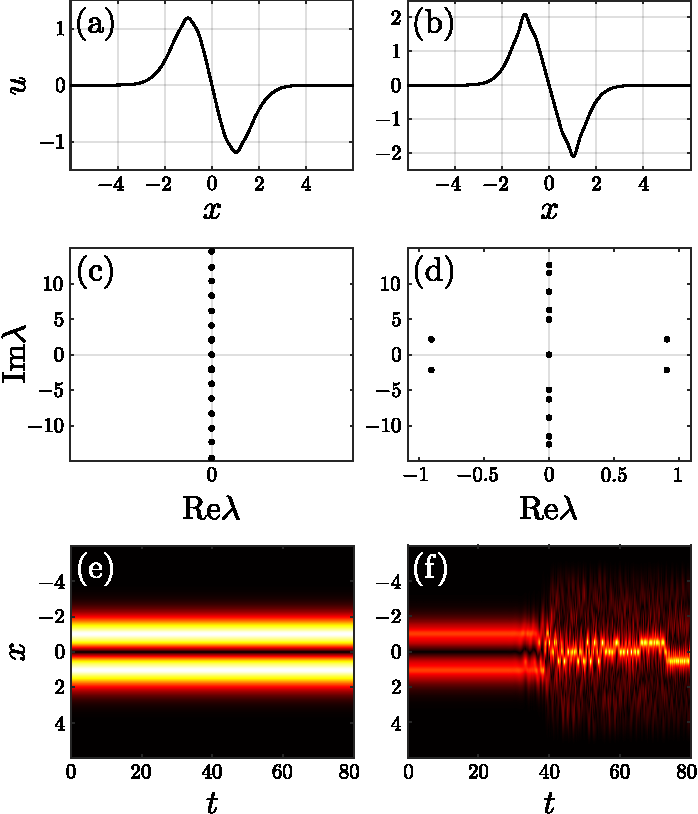
\includegraphics[scale = 1]{pic/stability, non-zero mean cosine nho}
	\caption{
		Results of stability analysis for solutions belonging to the branch $\Gamma_1$ of \eqref{eq:gpe-non-zero-mean} with pseudopotential $P(x) = 1 + 2 \cos (12 x)$, and different parameters of $\omega$.
		Shapes $u(x)$ of the stationary solutions are presented in panels (a) $\omega = 2$ and (b) $\omega = 0$.
		The linear-stability spectrums are in panels (c) and (d) correspondingly.
		The evolutionary simulations are presented in panels (e) and (f).
		Localized solution with parameter $\omega = 2$ is stable, while solutions with parameter $\omega = 0$ is unstable.
	}
\label{fig:stability-nho-non-zero-mean}
\end{figure}

\subsection{Periodic pseudopotential with Zero Mean, $|P_0| \ll |P_1|$}

According to the results of the previous section, the effect of a rapidly oscillating pseudopotential with non-zero mean may be approximated using the standard nonlinear harmonic-oscillator model with uniform nonlinearity.
However, the situation becomes essentially different for the case $|P_0| \ll |P_1|$.
If $P_0$ component of the pseudopotential can be neglected, we drop $P_0$, and rescale equation \eqref{eq:gpe-parabolic} by replacing
\begin{equation}
	\Psi \to \Psi / \sqrt{|P_1|},
\end{equation}
which leads to the equation
\begin{equation}
	i \Psi_t + \Psi_{xx} + x^2 \Psi + \sigma_1 \cos (\Omega x) |\Psi|^2 \Psi = 0,
\label{eq:gpe-zero-mean}
\end{equation}
where $\sigma_1 = P_1 / |P_1| = \mathrm{sign}(P_1)$.
Stationary states equation has the form
\begin{equation}
	u_{xx} + (\omega - x^2) u + \sigma_1 \cos (\Omega x) u^3 = 0.
\label{eq:nho-zero-mean}
\end{equation}
The $N(\omega)$ curves for \eqref{eq:nho-zero-mean} with $\sigma_1 = $ and $\Omega = 8$ are shown in Figure~\ref{fig:stability-nho-zero-mean}.
Here we again observe the branches $\Gamma_n$ bifurcating from the linear limit and various families without linear counterparts, see branches (a), (b), (b'), (c), (d) in Figure~\ref{fig:stability-nho-zero-mean}.
The branches $\Gamma_n$ feature stable and unstable segments.
Most part of the localized solutions without linear counterpart being unstable, however we found one branch  without linear counterpart, family (b) on the corresponding inset of Figure~\ref{fig:stability-nho-zero-mean}, that features small stability region.

\begin{figure}[h]
\centering
	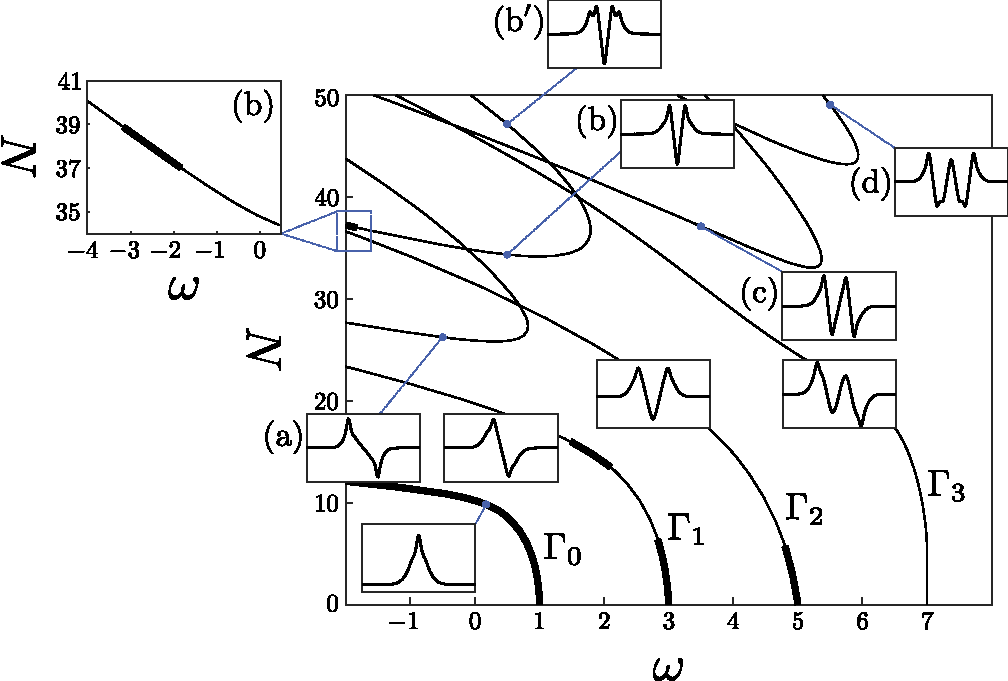
\includegraphics[scale = 1]{pic/branches for cosine nho, zero mean}
	\caption{
		Curves $N(\omega)$ for localized solutions of equation \eqref{eq:nho-zero-mean} with parameters $\sigma_1 = 1$ and $\Omega = 8$.
		Thin and bold lines show unstable and stable solution families.
		Insets depicts profiles of the solutions.
		Additional window in the upper left corner shows stability region for solutions from the branch (b) without linear counterpart.
	}
\label{fig:stability-nho-zero-mean}
\end{figure}

Let's focus on the localized solutions with linear counterpart under action of rapidly oscillating pseudopotential.
In the limit $N \\ 1$, weakly nonlinear solutions belonging to branches $\Gamma_n$, $n = 0, 1, \dots$, are produced by equations \eqref{eq:small-amplitude-expansion} where $\Delta_n$ is given by \eqref{eq:Delta_n}, with $P(x) = \sigma_1 \cos (\Omega x)$.
The numerical found values of $\Delta_n$, $n = 0, 1, 2$ for $\sigma_1$ and several different values of $\Omega$ are presented in Table~\ref{tab:Delta_n}.
\begin{table}[tbp]
\centering
\begin{tabular}{ccccc}
\hline
	$\Omega$ & \, 0 \, & \, 2 \, & \, 8 \, & \, 18 \\ \hline
	$n = 0$ & \, $3.9894 \cdot 10^{-1}$ \, & \, $2.4197 \cdot 10^{-1}$ \, & \, $1.3383 \cdot 10^{-4}$ \, & \, $1 \cdot 10^{-18}$ \\
	$n = 1$ & \, $2.9921 \cdot 10^{-1}$ \, & \, $-1.2100 \cdot 10^{-1}$ & $5.4536 \cdot 10^{-3} $ \, & \, $2 \cdot 10^{-15}$ \\
	$n = 2$ & \, $2.5557 \cdot 10^{-1}$ \, & \, $-1.3611 \cdot 10^{-1}$ \, & \, $2.1097 \cdot 10^{-2} $ \, & \, $5 \cdot 10^{-13}$ \\ \hline
\end{tabular}
\caption{
	The values of $\Delta _{n}$, $n = 0, 1, 2$, calculated as per Eq.~\eqref{eq:Delta_n} for $P(x) = \cos \left( \Omega x \right)$, $\Omega = 0, 2, 8, 18$.
	They determine the perturbative shift of chemical potential of weakly nonlinear localized solutions, pursuant to Eq.~\eqref{eq:small-amplitude-expansion}.
}
\label{tab:Delta_n}
\end{table}

To find the asymptotic form of $\Delta_n$ for $\Omega \to \infty$, we note that, for any arbitrary polynomial of degree $2m$
\begin{equation}
	Q_{2m}(x) = a_{2m} x^{2m} + a_{2m - 1} x^{2m - 1} + \dots + a_0,
\end{equation}
the following asymptotic relation holds
\begin{equation}
	\int \limits_{-\infty}^{+\infty} Q_{2m}(x) e^{-2 x^2} \cos (\Omega x)~dx \approx (-1)^m \frac{a_{2m} \sqrt{2 \pi} \Omega^{2m}}{2^{4m + 1}} e^{-\Omega^2 / 8}, \quad \Omega \to \infty.
\label{eq:polynomial-asymptotic}
\end{equation}
Since the coefficient in front of the highest-power term in the Hermite polynomial $H_n(x)$ is $2^n$, equation \eqref{eq:polynomial-asymptotic} with $Q_{2m}(x)$ substituted by  $H_n(x)$ yields
\begin{equation}
	\Delta_n \approx \frac{\sqrt{2} \Omega^{4n}}{2^{6n + 1} (n!)^2 \sqrt{\pi}} e^{-\Omega^2 / 8}, \quad \Omega \to \infty.
\label{eq:Delta_n-asymptotic}
\end{equation}
Therefore, for sufficiently large $\Omega$, $\Delta_n$ are all positive and decay exponentially, which agrees with the data in Table~\ref{tab:Delta_n}.

In the small-amplitude limit, the stability of localized solutions with linear counterpart is determined by the eigenvalues of matrix $\widetilde{M}_n$, see \eqref{eq:M}.
One can compute these eigenvalues numerically with any necessary accuracy.
The results for tow different values of frequency, $\Omega = 8$ and $\Omega = 16$, are summarized in Tables~\ref{tab:M-eigenvalues-8} and \ref{tab:M-eigenvalues-16}.
In these tables, $n$ is the index of the branch $\Gamma_n$.
For instance, $n = 2$ means that the brach $\Gamma_2$, which starts from $\tilde{\omega}_2 = 2 \cdot 2 + 1 = 5$, is under consideration.
While $k$, running from $0$ to $n - 1$, enumerates double eigenvalues $\widetilde{\Lambda}_k = 4(n - k)^2$.
Each cell with $n > k$ contains either tow real numbers or symbol ``$\mathbb{C}$''.
These number are real eigenvalues of matrix $\widetilde{M}_n$, whereas symbol ``$\mathbb{C}$'' indicates that eigenvalues of $\widetilde{M}_n$ are complex, and the corresponding low-amplitude solutions of the branch $\Gamma_n$ are unstable.
For $n < k$ the double eigenvalues do not exist (marked with dashes at the corresponding positions in the tables).

\begin{table}[tbp]
\centering
\begin{tabular}{cccccc}
\hline
	& \, $n = 1$ \, & \, $n = 2$ \, & \, $n = 3$ \, & \, $n = 4$ \, & \, $n = 5$ \\ \hline
	$k = 0$ & \, $\begin{array}{c} 0.132 \\ -0.028 \end{array}$ \, & \, $\begin{array}{c} -0.012 \\ 0.203 \end{array}$ \, & \, $\mathbb{C}$ \, & \, $\begin{array}{c} 0.424 \\ -0.828 \end{array}$ \, & \, $\begin{array}{c} -0.845 \\ -0.660 \end{array}$ \\ \hline
	$k = 1$ & \, $-$ \, & \, $\begin{array}{c} -0.176 \\ 0.159 \end{array}$ \, & \, $\begin{array}{c} 0.432 \\ -0.190 \end{array}$ \, & \, $\begin{array}{c} -0.486 \\ 0.048 \end{array}$ \, & \, $\begin{array}{c} 0.356 \\ 0.944 \end{array}$ \\ \hline
	$k = 2$ & \, $-$ \, & \, $-$ \, & \, $\begin{array}{c} -0.068 \\ -0.132 \end{array}$ \, & \, $\begin{array}{c} -0.206 \\ 0.196 \end{array}$ \, & \, $\begin{array}{c} 0.531 \\ -0.600 \end{array}$ \\ \hline
	$k = 3$ & \, $-$ \, & \, $-$ \, & \, $-$ \, & \, $\mathbb{C}$ \, & \, $\begin{array}{c} 0.166 \\ -0.122 \end{array}$ \\ \hline
	$k = 4$ & \, $-$ \, & \, $-$ \, & \, $-$ \, & \, $-$ \, & \, $\mathbb{C}$ \\ \hline
\end{tabular}
\caption{
	Eigenvalues of matrix $\widetilde{M}_n$ in the case $P(x) = \cos (8x)$.
	Here $n$ is the index of branch $\Gamma_n$, and $k$ enumerates double eigenvalues $\widetilde{\Lambda}_k = 4(n - k)^2$.
	Each cell with $n > k$ contains either tow real numbers or symbol ``$\mathbb{C}$''.
	These number are real eigenvalues of matrix $\widetilde{M}_n$, whereas symbol ``$\mathbb{C}$'' indicates that eigenvalues of $\widetilde{M}_n$ are complex, and the corresponding low-amplitude solutions of the branch $\Gamma_n$ are unstable.
	Results in this table agree with Figure~\ref{fig:stability-nho-zero-mean}.
}
\label{tab:M-eigenvalues-8}
\end{table}

% TODO: Check the values in the table. Possible there is mistake, $\Omega = 18$, not $16$.
\begin{table}[tbp]
\centering
\begin{tabular}{cccccc}
\hline
	& $n = 1$ & $n = 2$ & $n = 3$ & $n = 4$ & $n = 5$ \\ \hline
	$k = 0$ & $\begin{array}{c} -2.0 \cdot 10^{-11} \\ 5.7 \cdot 10^{-10} \end{array}$ & $\begin{array}{c} -7.6 \cdot 10^{-9} \\ -9.2 \cdot 10^{-7} \end{array}$ & $\begin{array}{c} -8.7 \cdot 10^{-7} \\ 2.2 \cdot 10^{-4} \end{array}$ & $\begin{array}{c} -4.0 \cdot 10^{-5} \\ -1.2 \cdot 10^{-2} \end{array}$ & $\begin{array}{c} -9.5 \cdot 10^{-4} \\ 1.5 \cdot 10^{-1} \end{array}$ \\ \hline
	$k = 1$ & $-$ & $\begin{array}{c} -4.2 \cdot 10^{-9} \\ 7.3 \cdot 10^{-8} \end{array}$ & $\begin{array}{c} -5.8 \cdot 10^{-7} \\ -3.6 \cdot 10^{-5} \end{array}$ & $\begin{array}{c} -3.0 \cdot 10^{-5} \\ 3.3 \cdot 10^{-3} \end{array}$ & $\begin{array}{c} -7.6 \cdot 10^{-4} \\ -6.8 \cdot 10^{-2} \end{array}$ \\ \hline
	$k = 2$ & $-$ & $-$ & $\begin{array}{c} -3.4 \cdot 10^{-7} \\ 3.9 \cdot 10^{-6} \end{array}$ & $\begin{array}{c} -2.0 \cdot 10^{-5} \\ -6.8 \cdot 10^{-4} \end{array}$ & $\begin{array}{c} -5.7 \cdot 10^{-4} \\ 2.6 \cdot 10^{-2} \end{array}$ \\ \hline
	$k = 3$ & $-$ & $-$ & $-$ & $\begin{array}{c} -1.3 \cdot 10^{-5} \\ 1.0 \cdot 10^{-4} \end{array}$ & $\begin{array}{c} -3.6 \cdot 10^{-4} \\ -6.8 \cdot 10^{-3} \end{array}$ \\ \hline
	$k = 4$ & $-$ & $-$ & $-$ & $-$ & $\begin{array}{c} -2.7 \cdot 10^{-4} \\ 1.5 \cdot 10^{-3} \end{array}$ \\ \hline
\end{tabular}
\caption{
	Eigenvalues of matrix $\widetilde{M}_n$ for $P(x) = \cos (16 x)$.
	The same notation as for Table~\ref{tab:M-eigenvalues-8} is used.
}
\label{tab:M-eigenvalues-16}
\end{table}

To be specific, let us describe in details the branch $\Gamma_2$ in the case of $P(x) = \cos (8x)$, Table~\ref{tab:M-eigenvalues-8}.
In this case, there are tow double eigenvalues in the spectrum, $\widetilde{\Lambda}_0 = 16$ and $\widetilde{\Lambda}_1 = 4$.
According to Table~\ref{tab:M-eigenvalues-8} and equation \eqref{eq:eigenvalues-split}, they split as
\begin{eqnarray}
	&& \Lambda_{0, 1} = 16 - 0.012 \cdot \varepsilon^2 + \dots, \quad \Lambda_{0, 2} = 16 + 0.203 \cdot \varepsilon^2 + \dots; \\
	&& \Lambda_{1, 1} = 4 - 0.176 \cdot \varepsilon^2 + \dots, \quad \Lambda_{1, 2} = 4 + 0.159 \cdot \varepsilon^2 + \dots.
\end{eqnarray}
Hence, the small-amplitude solutions belonging to branch $\Gamma_2$ are stable in this case.
The situation is different for branches $\Gamma_{3,4,5}$ from Table~\ref{tab:M-eigenvalues-8}.
For each of these branches the bifurcation of a complex-conjugate pair occurs: for $n = 3$ the eigenvalue $\widetilde{\Lambda}_0 = 36$ splits into complex eigenvalues, while for $n = 4$ and $n = 5$ the same happens for $\widetilde{\Lambda}_2 = 4$.
Therefore, for $\Omega = 8$ the small-amplitude solutions are stable  for branches $\Gamma_{0, 1, 2}$, but unstable for $\Gamma_{3, 4, 5}$.
Table~\ref{tab:M-eigenvalues-16} is produced for $\Omega = 16$.
It implies that the small-amplitude solutions are stable for all branches $\Gamma_{1, \dots, 5}$.

To explain the different stability of small-amplitude solutions with different values of frequency $\Omega$, we consider the behaviour of the eigenvalues of $\widetilde{M}_n$ at $\Omega \to \infty$.
Using explicit results given by equations \eqref{eq:Mn11}--\eqref{eq:Mn22} and asymptotic relation \eqref{eq:Delta_n-asymptotic}, we obtain
\begin{align}
\langle M_n \tilde{u}_k, \tilde{u}_k \rangle & \sim -\frac{2\sqrt{2} (n - k) \Omega^{4n}}{2^{6n} (n!)^2 \sqrt{\pi}} e^{-\Omega^2 / 8}; \\
\langle M_n \tilde{u}_k, \tilde{u}_{2n-k} \rangle = -\langle M_n \tilde{u}_{2n-k}, \tilde{u}_k \rangle & \sim \frac{2\sqrt{2} (n - k) \Omega^{4n}}{2^{6n} n! \sqrt{k! (2n - k)!} \sqrt{\pi}} e^{-\Omega^2 / 8}; \\
\langle M_n \tilde{u}_{2n-k}, \tilde{u}_{2n-k} \rangle & \sim -\frac{4\sqrt{2} (n - k) \Omega^{2(3n - k)}}{\sqrt{\pi} 2^{3 (3n - k)} n! (2n - k)!} e^{-\Omega^2 / 8}.
\end{align}
These relations imply that
\begin{equation}
	\widetilde{M}_n =
	\begin{pmatrix}
		O(\Omega^{4n} e^{-\Omega^2 / 8}) & O(\Omega^{4n} e^{-\Omega^2 / 8}) \\
		O(\Omega^{4n} e^{-\Omega^2 / 8}) & O(\Omega^{2(3n-k)} e^{-\Omega^2 / 8})
	\end{pmatrix},
	\quad \Omega \to \infty.
\end{equation}
All elements of the matrix $\widetilde{M}_n$ are of the same order, except for the one in the right lower corner which is of greater order since $n > k$.
It mean that, for $\Omega$ large enough, eigenvalues of $\widetilde{M}_n$ are real, hence the solutions from branches $\Gamma_n$ for arbitrary $n$ are stable in the small-amplitude limit.
This explains the difference between Table~\ref{tab:M-eigenvalues-8} and Table~\ref{tab:M-eigenvalues-16}.
The increase of the frequency from $\Omega = 8$ to $\Omega = 16$ results in stabilization of some small-amplitude solutions. 

Results of our asymptotic findings are illustrated in Figure~\ref{fig:branches-with-linear-counterpart-zero-mean}, where numerically generated $N(\omega)$ curves for $\Omega = 8$, $\Omega = 12$, and $\Omega = 16$ are depicted.
It follows from these plots that the branch $\Gamma_0$ is the ``most stable'' one for all the three values of $\Omega$.
One also notice that, for the greatest value $\Omega = 16$ there exist a ``stability window'' in a vicinity of the bifurcations for all branches $\Gamma_{0,1,2,3}$, in agreement with the asymptotic results presented above.

\begin{figure}[h]
\centering
	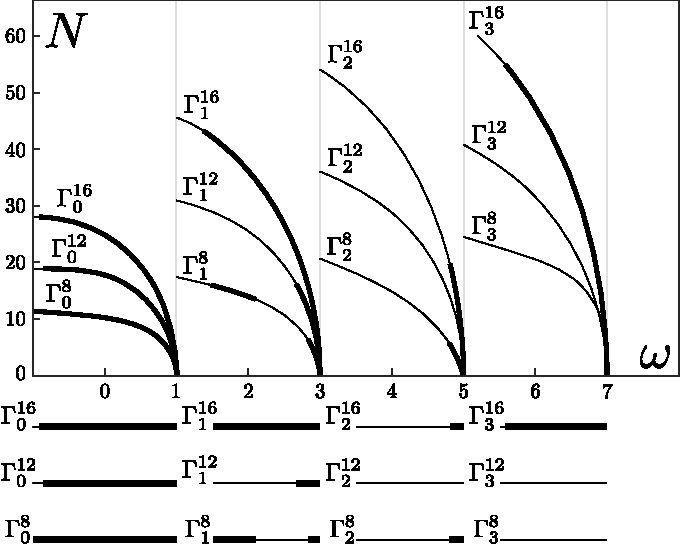
\includegraphics[scale = 1]{pic/branches with linear counterpart, zero mean cosine nho}
	\caption{
		Curves $N(\omega)$ of branches $\Gamma_n$, $n = 0, 1, 2, 3$ for equation \eqref{eq:nho-zero-mean} with $\sigma_1 = 1$ and $\Omega = 8, 12, 16$.
		The following notation is used: branch $\Gamma_n^{\Omega}$ corresponds to the branch with linear counterpart $\Gamma_n$, obtained for equation \eqref{eq:nho-zero-mean} where the frequency of pseudopotential equals $\Omega$.
		Bold (thin) lines correspond to stable (unstable) solutions.
		For convenience the stability of the families $\Gamma_n^{\Omega}$ is duplicated by straight lines under the main plot.
	}
\label{fig:branches-with-linear-counterpart-zero-mean}
\end{figure}

Numerical study of the temporal evolution of localized solutions in the framework of time-dependent GPE \eqref{eq:gpe-parabolic} confirms the prediction of the linear-stability analysis, see Figure~\ref{fig:stability-nho-zero-mean}.
As an example of a distinctive pattern of dynamical behaviour of unstable stationary solution under small perturbation, in Figure~\ref{fig:stability-nho-zero-mean} we display the transformation of an unstable solution from the branch $\Gamma_1$ into a pulsating object localized over one period of the pseudopotential $P(x) = \cos (8x)$.

\pagebreak
\begin{figure}[h]
\centering
	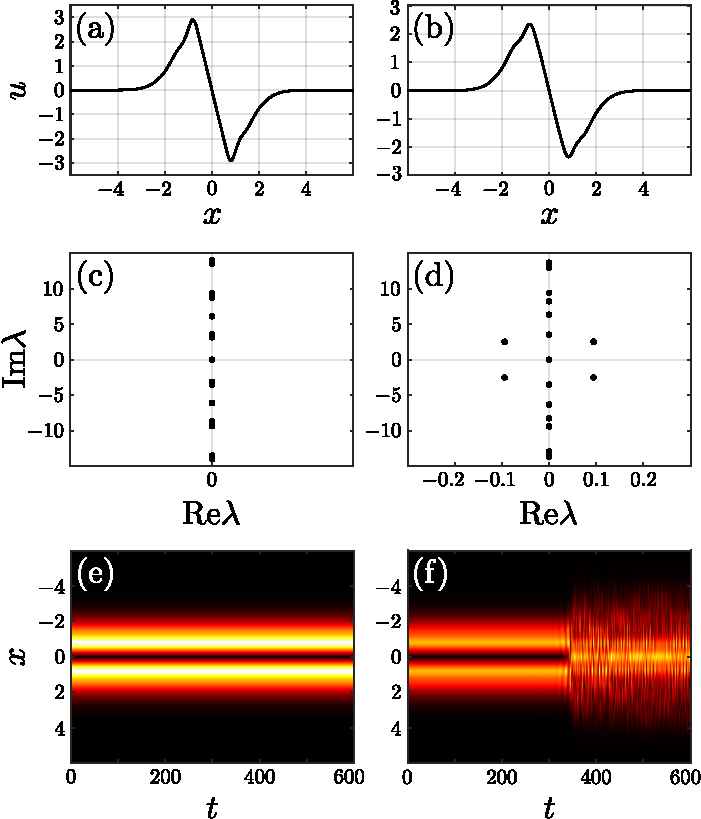
\includegraphics[scale = 1]{pic/stability, zero mean cosine nho}
	\caption{
		Results of stability analysis for solutions belonging to the branch $\Gamma_1$ of \eqref{eq:gpe-zero-mean} with pseudopotential $P(x) = \cos (8 x)$, and different parameters of $\omega$.
		Shapes $u(x)$ of the stationary solutions are presented in panels (a) $\omega = 2$ and (b) $\omega = 2.5$.
		The linear-stability spectrums are in panels (c) and (d) correspondingly.
		The evolutionary simulations are presented in panels (e) and (f).
		Localized solution with parameter $\omega = 2$ is stable, while solutions with parameter $\omega = 2.5$ is unstable.
	}
\label{fig:stability-nho-zero-mean}
\end{figure}
\pagebreak

\section{Summary}

In this chapter we studied localized stationary solutions of Gross--Pitaevskii equation with the harmonic-oscillator potential and pseudopotential $P(x)$, which is a periodic function oscillating with spatial frequency $\Omega$.
Let's summarize out results.
It was found that the presence of periodic pseudopotential significantly enrich the variety of localized solutions, in comparison with the well-studied case of the uniform nonlinearity \eqref{eq:nho}.
Specifically, GPE with periodic pseudopotential admits solutions without linear counterpart which do not exist in the case of $P(x) = \pm 1$.
As concerns solutions bifurcating from eigenstate of linear problem, their properties are essentially different depending on the presence constant additive term in $P(x)$ (non-zero mean value).
If the mean is non-zero, then properties of nonlinear solutions in a rapidly oscillating pseudopotential may be approximated using solutions for the standard nonlinear harmonic-oscillator model (with constant pseudopotential).
However, the reduction to the standard model with constant nonlinearity does not work for the system with zero-mean periodic pseudopotential.
Most interesting, in this we have found that the rapidly oscillating pseudopotential can stabilize small-amplitude localized solutions belonging to higher families, which are unstable in the model with $P(x)$ of non-zero mean.
Specifically, for any given branch with index $n$, there exists a threshold value of the spatial frequency $\Omega_n$, such that the small-amplitude solutions belonging to this branch are stable for $\Omega > \Omega_n$.
All results of our work were published in \cite{AlfimovGegelLebedevMalomedZezyulin}.
